% -*- mode: latex-mode; TeX-engine: xetex; LaTeX-command-style: (("" "SOURCE_DATE_EPOCH=0 %(PDF)%(latex) --shell-escape %S%(PDFout)")); TeX-master: "../dissertation.tex"; -*-

\chapter{Raman Sideband Cooling}
\label{ch:rsc}

\section{Introduction}
(In order to achieve full quantum control on molecules, we need to control atoms first.)
(An example of such control)
(Motional degrees of freedom)
(PGC cools to ...)
(RSC to further cool.)
\todo{Define abbreviation RSC}

\section{Basic Theory}
\label{ch:rsc-basic-theory}

\begin{figure}
  \centering
  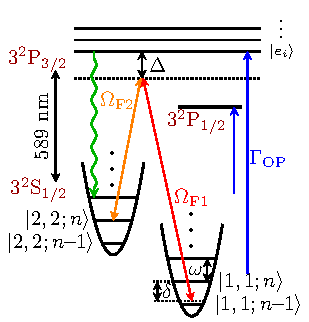
\includegraphics[width=8cm]{figures/na_rsc_schematics.pdf}
  \caption[Schematics of Raman sideband cooling for Sodium.]{
    Single Na atom Raman sideband cooling scheme.
    The Raman transitions couples $|2,2;n\rangle$ and $|1,1;n+\Delta n\rangle$
    through the intermediate states $|e_i\rangle$ in the $3^2P_{3/2}$ electronic states.
    The transitions have a one-photon detuning $\Delta_i\approx75$ GHz.
    Two-photon detuning, $\delta$, is defined relative to the $\Delta n=0$ carrier transition.
    For optical pumping, we use two $\sigma^+$ polarized transitions,
    one to pump the atom state out of $|1,1\rangle$ via $3^2P_{3/2}$
    and one to pump atoms out of $|2,1\rangle$ via $3^2P_{1/2}$
    to minimize heating of the $|2,2\rangle$ state.
    \label{fig:na-rsc-schematics}}
\end{figure}

The relevant energy diagram and the laser frequencies for RSC are shown in
Fig.~\ref{fig:na-rsc-schematics}.
We approximate the trapping potential using a harmonic oscillator.
Since this is a separable potential, we can use only the 1D motional state $|n\rangle$
and the result can be easily generalized to the full 3D system.

The cooling sequence consists of two types of pulses.
First, a Raman pulse drives the atom to a different hyperfine state while simultaneously
reduces the motional energy of the atom.
The optical pumping (OP) pulse afterwards then reset the hyperfine state of the atom
and reduce the entropy of the system.
In this section, we will discuss the theory of each types of pulses individually.
We will cover how the pulses affect cooling performance in section \ref{ch:rsc-challenges}.

\subsection{Raman Transition}
\label{ch:rsc-basic-theory-raman}

As shown in Fig.~\ref{fig:na-rsc-schematics},
the cooling sequence starts with the sodium atom in the
$|s_1\rangle\equiv|2,2\rangle$ hyperfine state,
and a Raman transition is used to drive the atom to the $|s_2\rangle\equiv|1,1\rangle$ state,
where $|F,m_F\rangle$ denotes the $F$ and $m_F$ quantum number for the sodium atom.
The full Rabi frequency for such a transition is given by
\begin{align*}
  \Omega_R^0=&\sum_{i}\frac{\Omega_{1i}\Omega_{2i}^*}{2\Delta_i}
\end{align*}
where the sum is over all the coupled excited states,
$\Omega_{ai}\equiv\langle a|\mathbf{d}\cdot\mathbf{E}_a|e_i\rangle$ is the single photon
Rabi frequency between $|a\rangle$ and $|e_i\rangle$
and $\Delta_i$ is the single photon detuning from excited state $|e_i\rangle$.

In order to account for the motional degrees of freedom, we need to include the spatial
wavefunction of the atom and light into account.
As mentioned above, we approximate the atomic motional wavefunction by the harmonic oscillator
eigenstates $|n\rangle$. Coupling between states different $n$ states from the Raman transition
is allowed due to the recoil from the Raman lasers,
which corresponds to a spacial phase imprinting of $\ue^{\ui\mathbf{\Delta k}\cdot\mathbf{\hat x}}$
where $\mathbf{\Delta k}$ is the wavevector difference between the two Raman beams.
Using the creation ($\hat a^\dagger$) and annihilation ($\hat a$) operators and the relation
$\mathbf{\hat x}=\mathbf{x}_0(\hat a+\hat a^\dagger)$ where $x_0=\sqrt{\hbar/2m\omega}$
is the harmonic oscillator length, the phase factor can be expressed as
$\ue^{\ui\eta_R(\hat a+\hat a^\dagger)}$ where $\eta_R\equiv\mathbf{\Delta k}\cdot\mathbf{x}_0$
is the Lamb-Dicke parameter for the Raman transition \todo{\cite{}}.
The matrix element between motional state $|n\rangle$ and $|n'\rangle$ is therefore,
\[ M_{n,n'}=\langle n|\ue^{\ui\eta_R(\hat a+\hat a^\dagger)}|n'\rangle \]
and the final Raman Rabi frequency between motional states $n$ and $n'$ is given by,
\[ \Omega_{R}^{n,n'}=M_{n,n'}\Omega_R^0 \]
For $n=n'$, this is called a carrier transition and the others are called sideband transitions.
If the final state is higher than the initial one, i.e. $n'>n$, it is a heating sideband.
Likewise, transitions with $n'<n$ are cooling sidebands.

A closed form result for $M_{n,n'}$ is given in \todo{\cite{}},
\[ M_{n,n'}=\ue^{\eta_R^2/2}\sqrt{\frac{n_<!}{n_>!}}\eta_R^{|n-n'|}L_{n_<}^{|n-n'|}(\eta_R^2) \]
where $n_<$ and $n_>$ are the lesser and greater, respectively, of $n$ and $n'$,
and $L_n^\alpha$ is the generalized Laguerre polynomial,
\[ L_n^\alpha(x)\equiv\sum_{m=0}^n(-1)^m\begin{pmatrix}n+\alpha\\n-m\end{pmatrix}\frac{x^m}{m!} \]

An important limit is the so-called Lamb-Dicke regime defined by $\eta_R^2(2n+1)\ll 1$.
In this case, we can approximate the phase factor in leading order of $\eta_R$,
\[ \ue^{\ui\eta_R(\hat a+\hat a^\dagger)}\approx1+\ui\eta_R(\hat a+\hat a^\dagger) \]
and the matrix element
\[ M_{n,n'}\approx\delta_{n,n'}+\ui\eta_R\sqrt{n+1}\delta_{n+1,n'}+\ui\eta_R\sqrt{n}\delta_{n,n'+1} \]
the three terms corresponds to the carrier ($n'=n$),
the first order heating sideband ($n'=n+1$)
and the first order cooling sideband ($n'=n-1$) with corresponding strength
$1$, $\eta_R\sqrt{n+1}$ and $\eta_R\sqrt{n}$.
We can clearly see from this approximation that the coupling to other motional state
is stronger for a larger $\eta_R$ and higher motional quantum number $n$.
We will discuss this effect outside the Lamb-Dicke regime and its implication
on the cooling performance in more detail in section \ref{ch:rsc-challenges}.

\subsection{Optical Pumping}
\label{ch:rsc-basic-theory-op}

Driving the system on a cooling sideband with Raman transition can reduce the
motional energy of the atom. However, this is a fully coherent process that does
not reduce the system entropy and is not really ``cooling'' the system
or achieving better control on the quantum state of the system.
Instead, quantum state control is achieved in the RSC via the OP pulse.
The initial hyperfine state $|2,2\rangle$ is a stretched state so it is the
state the system naturally ends up in when $\sigma^+$ light is applied.
However, if this is done using scattering from a $F=2$ to $F'=3$ transition,
the OP beam will allow continuous photon cycle
between the $|2,2\rangle$ and the $|3',3\rangle$ causing unnecessary motional heating during OP.
Therefore, the OP must be done on a $F=2$ to $F'=2$ transition.
Unfortunately, for Na, the corresponding transition from $3^2S_{1/2}$ to $3^2P_{3/2}$
that is used for the MOT is not useable due to the small energy difference of
$60 \mathrm{MHz}$ (or $6$ line widths) between the $F'=2$ and $F'=3$ states
\cite{steck_sodium_nodate}.
Instead, we must use the sodium $\mathrm{D1}$ line, i.e. $3^2S_{1/2}$ to $3^2P_{1/2}$ transition,
which lacks a $F'=3$ excited state.
The $\mathrm{D1}$ light with $\sigma^+$ polarization is only used to pump atoms from
$F=2$ states (in particular $|2,1\rangle$ which is populated during the OP process).
Since the goal of the OP pulse is to clear the atom population in all states but $|2,2\rangle$,
the photon cycling is not a concern for $F=1$ states and the $\mathrm{D2}$ line
is used for OP of $F=1$ states instead.
This also allow us to reuse the MOT light source and simplifies our setup.

\section{Setup}

\ref{fig:na-rsc-geometry}

\begin{figure}
  \centering
  \includegraphics[width=8cm]{figures/na_rsc_geometry.pdf}
  \caption[Beams and field geometry for Sodium Raman sideband cooling]{
    Geometry and polarizations of the Raman and optical pumping beams relative to the
    optical tweezer and bias magnetic field.
    Raman beams R1 and R4 address the radial $x$-mode.
    R1 and R2 address the radial $y$-mode.
    R3 and R4 address the axial $z$-mode, where the beams also couple to radial motion,
    but this coupling can be neglected when the atoms is cooled to the ground state of motion.
    \label{fig:na-rsc-geometry}}
\end{figure}

\section{Cooling Performance and Challenge with Large Lamb-Dicke Parameter}
\label{ch:rsc-challenges}

\ref{fig:na-rsc-challenges}

\begin{figure}
  \centering
  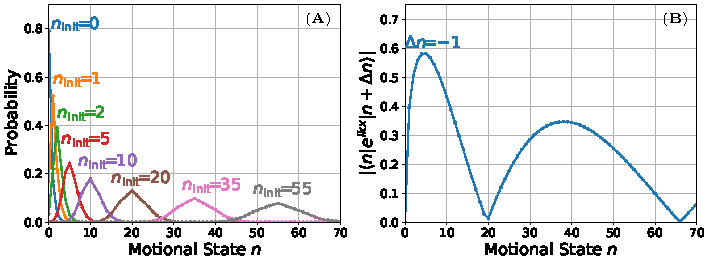
\includegraphics[width=\textwidth]{figures/na_rsc_challenges.pdf}
  \caption[Optical pumping motional-state redistribution and Raman coupling]{
    Optical pumping motional-state redistribution and Raman coupling for large LD parameters
    for the axial direction ($z$).
    The range plotted covers $95$\% of the initial thermal distribution.
    (A) Motional state distribution after one OP cycle for different initial states motion,
    $n_{\textrm{init}}$.
    Due to photon-recoil and the large LD parameter, $\eta^{\textrm{OP}}_z=0.55$,
    there is a high probability of $n$ changing.
    (B) Matrix elements for Raman transition on the first order cooling sideband
    deviate from $\sqrt{n}$ scaling with multiple minima.
    \label{fig:na-rsc-challenges}}
\end{figure}

\section{Solution: High Order Sidebands}

\ref{fig:na-rsc-mele-raman}

\begin{figure}
  \centering
  \includegraphics[width=8cm]{figures/na_rsc_mele_raman.pdf}
  \caption[Raman coupling including high order sidebands]{
    Matrix elements for Raman transition including high order sidebands.
    During cooling, we utilize the fact that high motional states couple most effectively
    to sidebands with large $|\Delta n|$ in order to overcome the issue with
    variation and dead zone in the coupling strengths.
    \label{fig:na-rsc-mele-raman}}
\end{figure}

\section{Solution: Simulation Based Optimization}

\ref{fig:na-rsc-sequence}

\begin{figure}
  \centering
  \includegraphics[width=\textwidth]{figures/na_rsc_sequence.pdf}
  \caption[Simulation optimized Raman sideband cooling sequence for Sodium]{
    Schematic of the cooling pulse sequence. The tweezer is strobed at 3 MHz to
    reduce light shifts during optical pumping~\cite{hutzler_eliminating_2017}.
    Each cooling cycle consists of $8$ sideband pulses.
    The four axial pulses address two sideband orders.
    The two pulses in each radial direction either address $\Delta n=-2$ and $\Delta n=-1$
    or have different durations to drive $\Delta n=-1$,
    at the end of the cooling sequence when most of the population is below $n=3$.
    The Raman cooling and spectroscopy pulses have Blackman envelopes~\cite{kasevich_laser_1992}
    to reduce off-resonant coupling,
    while the measurement Rabi pulses in Fig.~\ref{fig:na-rsc-rabi-flop}
    have square envelopes to simplify analysis.
    \label{fig:na-rsc-sequence}}
\end{figure}

\section{Calibration}
(Sideband/carrier)\todo{Use scattering to calibrate intensity}
(Cold vs hot)

\section{Cooling Performance}

\ref{fig:na-rsc-spectrum}
\ref{fig:na-rsc-rabi-flop}

\begin{figure}
  \centering
  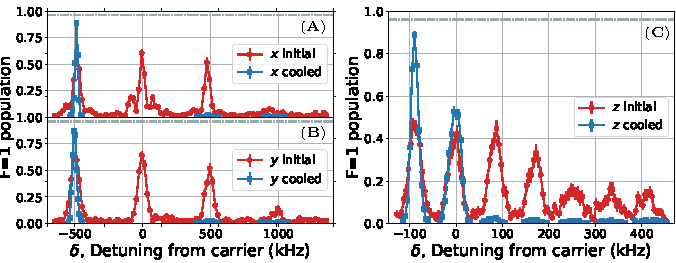
\includegraphics[width=\textwidth]{figures/na_rsc_spectrum.pdf}
  \caption[Raman sideband spectra before and after cooling]{
    Raman sideband spectra for (A) $x$, (B) $y$, (C) $z$ axis before (red circle)
    and after (blue square) applying Raman sideband cooling sequence.
    The height of the cooling sidebands (positive detuning)
    are strongly suppressed after cooling which suggests most of the atoms are cooled
    to the motional ground state in the trap.
    \label{fig:na-rsc-spectrum}}
\end{figure}

\begin{FPfigure}
  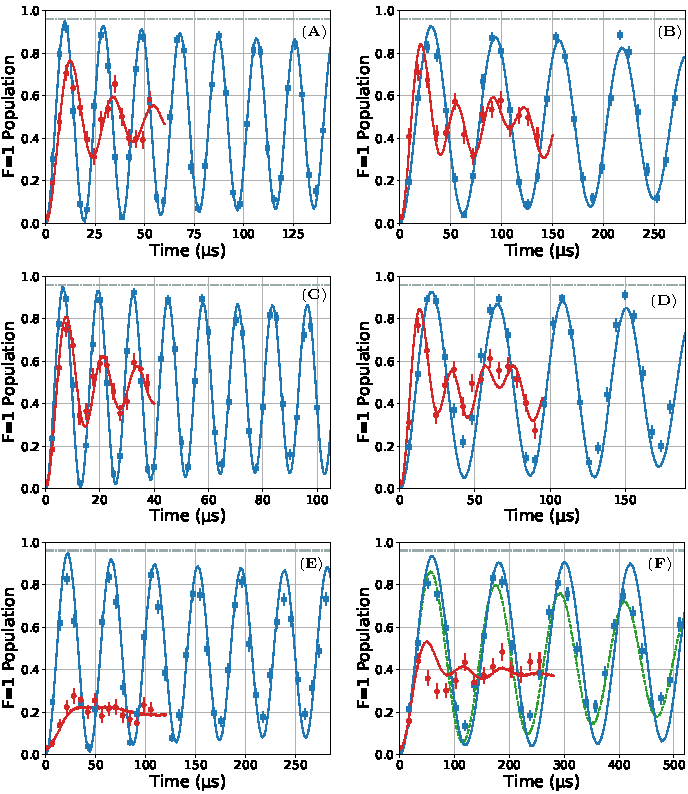
\includegraphics[width=\textwidth]{figures/na_rsc_rabi_flop.pdf}
  \caption[Rabi flopping on carriers and sidebands]{
    Rabi flopping on radial axis $x$ (A) carrier and (B) $\Delta n_x=1$ sideband,
    radial axis $y$ (C) carrier and (D) $\Delta n_x=1$ sideband,
    axial axis $z$ (E) carrier and (F) $\Delta n_x=1$ sideband,
    before (red circle) and after (blue square) Raman sideband cooling.

    Solid lines (both red and blue) in all plots are fits to a Rabi-flopping
    that includes a thermal distribution of motional states~\cite{meekhof_generation_1996}
    as well as off-resonant scattering from the Raman beams.

    The blue lines correspond to a ground state probability of (A-D) $98.1$\% along radial axis
    and (E-F) $95$\% along the axial axis after cooling.
    The red lines correspond to a thermal distribution of $80$ $\mu$K before RSC.
    The horizontal dashed lines in all the plots correspond to the $4\,\%$ probability
    of imaging loss.

    The green dashed line in (F) includes the additional decoherence due to
    a fluctuation of the hyperfine splitting of magnitude $3$ kHz.
    We see that the decoherence effect is strongest for the post-cooling data on
    the axial $\Delta n_z=1$ sideband where the Rabi frequency is the lowest.
    \label{fig:na-rsc-rabi-flop}}
\end{FPfigure}
\afterpage{\clearpage}
